% -----------------------------------------------
% Template for SMC 2022
% based on SMC 2022 template
% -----------------------------------------------

\documentclass{article}
\usepackage{smc}
\usepackage{times}
\usepackage{ifpdf}
\usepackage[english]{babel}
\usepackage{cite}
%%%% Added by LR
\usepackage{booktabs}
\usepackage{makecell}

%%%%%%%%%%%%%%%%%%%%%%%% Some useful packages %%%%%%%%%%%%%%%%%%%%%%%%%%%%%%%
%%%%%%%%%%%%%%%%%%%%%%%% See related documentation %%%%%%%%%%%%%%%%%%%%%%%%%%
%\usepackage{amsmath} % popular packages from Am. Math. Soc. Please use the 
%\usepackage{amssymb} % related math environments (split, subequation, cases,
%\usepackage{amsfonts}% multline, etc.)
%\usepackage{bm}      % Bold Math package, defines the command \bf{}
%\usepackage{paralist}% extended list environments
%%subfig.sty is the modern replacement for subfigure.sty. However, subfig.sty 
%%requires and automatically loads caption.sty which overrides class handling 
%%of captions. To prevent this problem, preload caption.sty with caption=false 
%\usepackage[caption=false]{caption}
%\usepackage[font=footnotesize]{subfig}


%user defined variables
\def\papertitle{GIHME : Dataset of Guitar Improvisations with Hexaphonic Muti-Effects}
\def\firstauthor{Loïc Reboursière}
\def\secondauthor{Second author}
\def\thirdauthor{Third author}

% adds the automatic
% Saves a lot of output space in PDF... after conversion with the distiller
% Delete if you cannot get PS fonts working on your system.

% pdf-tex settings: detect automatically if run by latex or pdflatex
\newif\ifpdf
\ifx\pdfoutput\relax
\else
   \ifcase\pdfoutput
      \pdffalse
   \else
      \pdftrue
\fi

\ifpdf % compiling with pdflatex
  \usepackage[pdftex,
    pdftitle={\papertitle},
    pdfauthor={\firstauthor, \secondauthor, \thirdauthor},
    bookmarksnumbered, % use section numbers with bookmarks
    pdfstartview=XYZ % start with zoom=100% instead of full screen; 
                     % especially useful if working with a big screen :-)
   ]{hyperref}
  %\pdfcompresslevel=9

  \usepackage[pdftex]{graphicx}
  % declare the path(s) where your graphic files are and their extensions so 
  %you won't have to specify these with every instance of \includegraphics
  \graphicspath{{./figures/}}
  \DeclareGraphicsExtensions{.pdf,.jpeg,.png}

  \usepackage[figure,table]{hypcap}

\else % compiling with latex
  \usepackage[dvips,
    bookmarksnumbered, % use section numbers with bookmarks
    pdfstartview=XYZ % start with zoom=100% instead of full screen
  ]{hyperref}  % hyperrefs are active in the pdf file after conversion

  \usepackage[dvips]{epsfig,graphicx}
  % declare the path(s) where your graphic files are and their extensions so 
  %you won't have to specify these with every instance of \includegraphics
  \graphicspath{{./figures/}}
  \DeclareGraphicsExtensions{.eps}

  \usepackage[figure,table]{hypcap}
\fi

%setup the hyperref package - make the links black without a surrounding frame
\hypersetup{
    colorlinks,%
    citecolor=black,%
    filecolor=black,%
    linkcolor=black,%
    urlcolor=black
}


% Title.
% ------
\title{\papertitle}

% Authors
% Please note that submissions are NOT anonymous, therefore 
% authors' names have to be VISIBLE in your manuscript. 
%
% Single address
% To use with only one author or several with the same address
% ---------------
%\oneauthor
%   {\firstauthor} {Affiliation1 \\ %
%     {\tt \href{mailto:author1@smcnetwork.org}{author1@smcnetwork.org}}}

%Two addresses
%--------------
% \twoauthors
%   {\firstauthor} {Affiliation1 \\ %
%     {\tt \href{mailto:author1@smcnetwork.org}{author1@smcnetwork.org}}}
%   {\secondauthor} {Affiliation2 \\ %
%     {\tt \href{mailto:author2@smcnetwork.org}{author2@smcnetwork.org}}}

% Three addresses
% --------------
 \threeauthors
   {\firstauthor} {ISIA Lab, UMONS \\ %
     {\tt \href{mailto:loic.reboursiere@umons.ac.be}{loic.reboursiere@umons.ac.be}}}
   {\secondauthor} {Affiliation2 \\ %
     {\tt \href{mailto:author2@smcnetwork.org}{author2@smcnetwork.org}}}
   {\thirdauthor} { Affiliation3 \\ %
     {\tt \href{mailto:author3@smcnetwork.org}{author3@smcnetwork.org}}}


% ***************************************** the document starts here ***************
\begin{document}
%
\capstartfalse
\maketitle
\capstarttrue
%
\begin{abstract}
This paper presents a novel guitar dataset made out of richtly annotated guitarists improvisations. The annotations gather notes, playing techniques, 
%(and extended techniques when used)
instrument tuning, audio effects configurations as well as transcription of post improvisations interviews. The dataset gathers ten hours of improvisations and around five hours of interviews. Those accompanying data make this dataset suitable for a variety of different research domains : from MIR to improvisation analysis and musicology. The recordings yielded to this dataset were done in the context of an hexaphonic multi-effect pratice study. Such a multi-effects is meant to work with an hexaphonic guitar (one pickup per string guitar) and grant the player with independant strings audio effects configurations. 
%An hexaphonic guitar is an electric (or electrified) guitar equipped with six individual pickups (one per string), aka an hexaphonic pickup.  
 This paper presents the dataset and the experiments it has been gathered from.  It also details, based the interviews transcriptions, a first analysis of the hexaphonic setup specificities regarding to the guitarists own practices. 
%This dataset

%10 hours of improvisations and around 5 hours of interviews have been recorded (audio and video). Those interviews gather guitarists feedbacks taken right after the improvisations and have been transcribed. Additional annotations such as played notes, used tunings or effects activation segments complete the dataset in order to provide keys to analyze how this kind of effects and instrument impact the guitarists' practices.

\end{abstract}
%

\section{Introduction}\label{sec:introduction}

hex guitar 
	> hex analysis/processing 
		> use of dataset 
			> duality
			> type of annotations
				> notes
				> fx config and activation/deactivation 
				> itw
			> while still work to be done on playing annotations tests on visualisation of such amount of info will be shown	
			

An hexaphonic guitar is an electric or acoustic guitar equipped with an hexaphonic pickup. This device gathers six individual pickups, one per string. As a result, six audio signals are available for further processing. As a comparison, on regular electric guitars, monophonic pickups mix the sound of all resonating strings down to one audio signal. With such system, different audio effects or analysis tools can be applied to each string independently. This type of pickups appeared in the late 1970s with guitar synthesizers which as the name implies correspond to guitars that can control synthesizers. On this type of instrument, hexaphonic pickups are of great help in converting notes to control signals, because they narrow down the complexity of pitch detection from polyphonic to six monophonic algorithms running in parallel. Apart from that main commercially-developped use case, hexaphonic pickups enable independent-string audio processing. The first physical units integrating individual string processing appeared at the end of the 1970s (ARP Avatar\footnote{\url{http://www.vintagesynth.com/arp/avatar.php}}, Matthias Gob's Paradis PolyDistorsion\footnote{\url{https://matthiasgrob.org/pEE/sndhist.htm}}, Keith McMillen's Zeta PolyFuzz\footnote{\url{http://www.keithmcmillen.com/wp-content/uploads/2014/12/keith_mcmillen_timeline.pdf}}, Roland GR100\footnote{\url{https://www.joness.com/gr300/GR-100.htm}} but, despite the large amount of creative potential it seems to have, hexaphonic audio processing has never reach a larger audience and remained a niche. 

This series of experiments and the resulting dataset\footnote{Which can be found online at : ANONYMIZED} were made to try to understand how individual string processing affects the guitarists practices and how guitarists can integrate a device which fosters polyphony and multitimbrality\footnote{Polyphony and multitimbrality both refer to the ability to distinguish in a piece of music several instruments or timbres. As sounds of strings of an hexaphonic guitar are separated, different timbres can easily be obtained by applying different effects with/without different settings therefore leading to multitimbrality.} in their practice and how it changes their practices or not. 

%%%%% Not sure to be left here
5 guitarists whose practices range from rock to contemporary music passing through jazz, improvisation and progressive rock have each followed a set of predefined scenarios during 3 days. 
While the second part list the various realted work, third part detailed the experimental structure and process. Fourth part gathers the different media composing the dataset. Finally, part five proposes a first analysis of the interviews material and part six detailed future works. 

It has to be noticed that, while this dataset was made to analyse the resulting practice of hexaphonic audio processing in improvisation context, the accompanying annotations (notes, tunings, effects segments activation) can make this dataset suited to more specifically Music Information Retrieval (MIR) -oriented tasks such as onsets detection, polyphonic pitch estimation, chord detection, etc.

\section{Related works}

Add detail info on available datasets, compared to actual annotations

Music datasets are mostly built and used in MIR-related contexts.  Some contains multiple types of musical instruments \cite{thickstun2017learning}, and some are oriented towards specific instrument such as the piano (\cite{Emiya2010MAPS},\cite{hawthorne2018enabling}) or the guitar (\cite{Kehling2014}, \cite{Author:Xi2018}). Most of these datasets are built for pitch detection but some of them are made for tasks such as guitar playing techniques \cite{Author:Su2014a}, chords \cite{nadar2019Chords}, effects \cite{Stein2010} and playing modes detection \cite{Foulon2014}. 

Apart from these datasets which were built to improve existing results on the MIR-related tasks previously listed, some are built to study musical and instrumental practices such as the Weimar Jazz Database\cite{Pfleiderer:2017:BOOK} from the Jazzomat project\cite{Frieler:2013:Jazzomat} which uses different MIR techniques to extract relevant information to describe and classify jazz improvisations. 

As mentioned above, the dataset presented in this paper goes a bit further by proposing recordings of guitarists' improvisations made using an hexaphonic multi-effects audio program. First hexaphonic effects appear in the late 1970s and beginning of the 1980s. The ARP Avatar\footnote{\url{http://www.vintagesynth.com/arp/avatar.php}} guitar synthesizer and the Roland GR-100\cite{joness-gr100} both includes an hexaphonic distorsion effects while the GR-300\cite{joness-gr300} integrates an hexaphonic harmonizer. Apart from this already established companies, entrepreneur Keith McMillen developed the PolyFuzz\cite{McMillen2015-timeline} guitar pedal (used by guitarist John Abercrombie) which integrates distorsion, fuzz and suboctave effects. Swiss Luthier Matthias Grob developed around the same period its PolyDistorsion \cite{grob:paradisGuitar} followed by a  multi-effects.
More recently in the research field, several works tackle the development of hexaphonic audio processing tools (\cite{sci:Puckette2007}, \cite{sci:Reboursiere2010} and their use in performance context \cite{Reboursiere2020_Puzzle_eng}\footnote{Sound recordings of hexaphonic effects can be found online, \href{https://soundcloud.com/medicationtime/sets/hexaphonic-effects}{https://soundcloud.com/medicationtime/sets/hexaphonic-effects}}.

How does GIHME fits into existing dataset, annotations and hex fx used
\section{Experiment structure}

Analysis of hexaphonic guitar pratices has been done in various artistic contexts \cite{Bates2009, sci:Graham2010}, some of them including the use of an hexaphonic multi-effects\cite{sci:Reboursiere2021_Phd}.
The experiment presented here was built up to investigate specific uses of hexaphonic pickup and multi-effetcs, especially the distribution of audio effects on specific groups of strings and the control of individual bypasses of the audio effects. 
For this experiment, five guitarists have been recorded playing the hexaphonic multi-effects on specific pre-defined scenarios. Four of them are professional guitarists and/or composers and/or improvisers and the last one is an amateur guitarist/composer\footnote{\href{https://www.youtube.com/channel/UCLHyrUsYR-gE5r\_4Vs45xkQ}{https://www.youtube.com/channel/UCLHyrUsYR-gE5r\_4Vs45xkQ}}. The four professional guitarists are part of a collective of musicians\footnote{\href{https://muzzix.info/}{https://muzzix.info/}} whose musical projects range from jazz and improvisation, to contemporary and prepared instruments while the amateur guitarist mostly evolves in rock style related music. In the rest of the paper we'll be referring to the guitarists using number from 1 to 5, 5 being the amateur guitarist. 

\subsection{Hexaphonic multi-effects}

The hexaphonic multi-effects used in these experiments is depicted in figure \ref{fig:hex-multi-effects}. It has been developped using Cycling' 74 Max MSP software. The multi-effects gathers four main elements : six hexaphonic audio effects, a bypass matrix gathering effects individual bypasses, a routing system to define effects order, an output mixer to adjust strings outputs individually. In order to limit the amount of new elements the guitarists had to digest during these experiments, the audio effects (overdrive, delay, ring modulation, flanger, tremolo, reverb) were chosen, arguably, among the most common for electric guitarists. Each of the effects display six instances (depicted by graphical colorful sliders) of each of its parameters, a preset system and individual bypasses. 
Those individual bypasses are gathered and developped graphically (bottom right part of the patch), forming a 6x6 graphical matrix that more easily gives feedback to the guitarist using scenario 2 foot controller. 
The effects routing system follows by default the order of the effects listed above but could be changed by the guitarist if it was needed.

\subsection{Pre-defined scenarios}
The whole process of this experiment go through the 3 following scenarios:
\begin{itemize}
    \item The first scenario is a "discovery scenario" where the guitarist, with the aid of the researcher, tests each hexaphonic effects, builds presets and create a "global sound" (i.e. chain of chosen effects and presets) to start working on the next scenario. No improvisation was recorded during this scenario.  
    
    \item The second scenario tackles \textit{the inherent polyphonic property of the hexaphonic pickup} by applying the chosen "global sound" to different groups of strings while the remaining strings are left dry (i.e. without any effects).
    
    \item The third scenario studies how this setup can be controlled in a performance context. A generic MIDI foot controller (Behringer FCB1010\footnote{\label{foot:Behringer1010}This controller provides ten buttons (configured with on/off behaviours) which can be linked to different mapping configurations (also called pages or banks in this type of devices). The browsing (going up or down) of this list of configurations can be done by two other buttons. Two continuous foot controller are also present on the device but were not used in the context of these experiments.}) was used to control different granularities of individual audio effects bypass controls (e.g, global effect bypass versus string-independent bypass control). 
\end{itemize} 
As a matter of clarity, the "discovery scenario" was named scenario 0 and the two remaining, respectively, scenario 1 and scenario 2.

\subsection{Scenarios 1 and 2 protocol}
Scenarios 1 and 2 follow the same protocol: 
\begin{itemize}
    \item They are made out of five sub-scenarios;
    \item Each sub-scenario are made of three steps: 
    \begin{itemize}
        \item Test : the guitarist plays with the proposed sub-scenario 's configuration and tries to develop musical ideas that can be used during the improvisation;
        \item Record : once the guitarist is satisfied with its findings, he records an improvisation of 3 to 4 minutes minimum (the longest being 18 minutes);
        \item Interview : the guitarist and the researcher talk about specific elements of the improvisation that was just recorded.
    \end{itemize}
    \item The two last steps can be repeated any amount of times the guitarist feels like, leading to try out different presets (i.e. changing the "global sound" to fit one specific sub-scenario) and/or different modes of playing;
    \item While the four first sub-scenarios are pre-defined, the fifth one is built by the guitarist. In scenario 1, the guitarist can choose the group of strings on which the ``global sound" can be applied. In scenario 2, the guitarist can decide which bypass control configuration he wants and create presets.
\end{itemize}

Table \ref{tab:scenario1} and \ref{tab:scenario2} summarize the different configurations of the sub-scenarios contained in each scenario.
While sub-scenarios 1\_1 and 1\_2 uses separation between "low" and "high" strings which is already used by guitarists in different playing styles\footnote{We can think e.g of acoustic blues style where guitarists often plays the accompaniement part on the low strings (often with alternating bass technique) and the melody on the high strings.}
It has to be noted that sub-scenarios 2\_3 and 2\_4 come out of the foot controller structure. As only ten buttons\footnote{See footnote \ref{foot:Behringer1010}} are available at once on the controller, mapping strategies needed to be defined in order to access the 36 individual bypasses of the multi-effects.  Another setup, e.g with 2 Voes MX-18 controllers\footnote{\href{https://www.voes.be/mx18.html}{https://www.voes.be/mx18.html}} (which we didn't know of at the time of the experiment), may have only need one sub-scenario to access the 36 individual bypasses controls.

\begin{table}
  
  \label{tab:scenario1}
  \begin{tabular}{ccc}
    \toprule
    Name &Strings with effects&Strings with no effect\\
    \midrule
    1\_1 & E-A-D & G-B-e\\
    1\_2 & G-B-e& E-A-D\\
    1\_3 & E-D-B & A-G-e\\
    1\_4 & A-G-e& E-D-B\\
    1\_5 & \multicolumn{2}{c}{Distribution (2\_3 or 2\_4) chosen by the \newline guitarist and definition of recallable presets}  \\
  \bottomrule
\end{tabular}
	\caption{Scenario 1 sub-scenarios.}
\end{table}

\begin{table}
  
  \label{tab:scenario2}
  \begin{tabular}{cc}
    \toprule
    Name & Bypass controls mappings\\
    \midrule
    2\_1 & 1 button controls the bypass of 1 hexaphonic \\
    & effect on all strings\\
    2\_2 & 1 button controls the bypass of the effects \\
    & applied on 1 string \\
    2\_3 & 1 bank per effect and 1 button per string\\
    2\_4 & 1 bank per string and 1 button per effect\\
    2\_5 & Distribution chosen by the guitarist  \\
  \bottomrule
\end{tabular}
	\caption{Scenario 2 sub-scenarios.}

\end{table}


\section{Recording process}
The audio processing setup is made out of several components : 
\begin{itemize}
    \item Two Godin guitars equipped with RMC hexaphonic piezo-electric pickups were at the disposal of the guitarists. 
    The first one, a Godin Mutliac, is a nylon-string guitar whereas the second one, a Godin LGXT, is a steel-string 
    guitar. Only one of the guitarist tried the first one, but eventually felt more at ease with the second one.
    \item A homemade breakout box is used to power pickup electronics and to convert the standard 13-pin din connecor 
    used for those pickups to 6 standard monophonic 6.35mm female Jack cable. 
    \item The breakout box is connected to an RME Fireface UCX soundcard throught 6 mono Jack cables. Sampling rate was 
    set to 44100 Hz and 32 bits of precision were used. 
    \item The hexaphonic multi-effects has been developed as a Max MSP patch (see Figure \ref{fig:hex-multi-effects}). This patch is an adapted version of the 
    one presented in \cite{Reboursiere2020_Puzzle_eng}. It gathers hexaphonic version of 6 well-known types of effects : 
    distorsion, delay, ring-modulator, flanger, tremolo and reverb as well as a matrix of individual bypass 
    control for each effect on each string. The effects were chosen in order not to add more newness to the hexaphony 
    itself. 
    \item Patch hexaphonic outputs are then connected to a mixing desk and to a quadriphonic speaker system with a 
    subwoofer. This diffusion system was the one present in the recording room and cannot be moved, but no specific
    spatialisation was used as this part of the hexaphonic process was not the subject of this experiment. Resulting Sounds 
    of the six strings were all equally broadcast on each speaker.
\end{itemize}

\begin{figure}
    \centering
    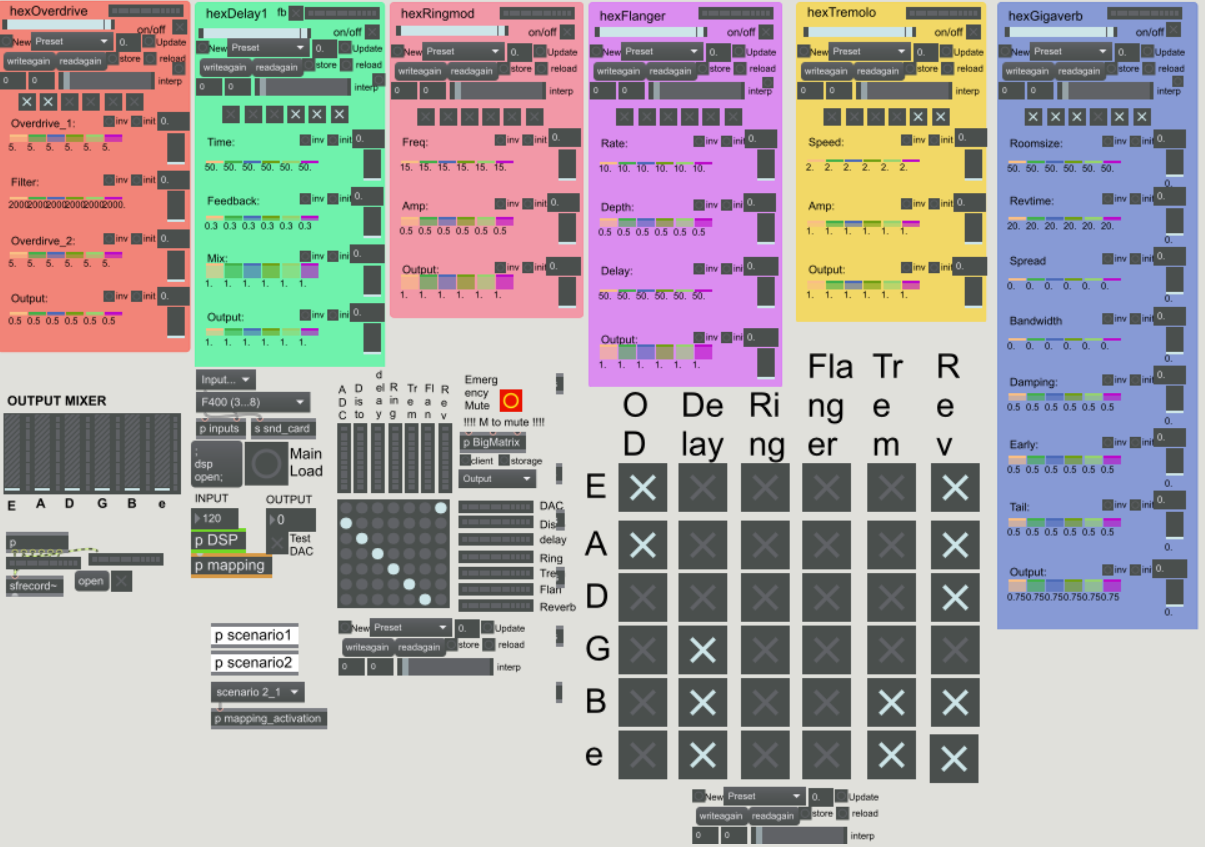
\includegraphics[scale=0.3]{figures/191025-Patch-experience.png}
    \caption{Hexaphonic Multi-Effects used for the experiments.}
    \label{fig:hex-multi-effects}
\end{figure}

Multiple audio and video files were recorded during the experiment. 
On the audio side, the hexaphonic audio signals were recorded before they hit the chosen effects and after they passed through the chosen effects. The first one enables to easily use any type of algorithm detection and the second one gives a detailed look at the produced sound. Moreover, the guitarist was asked to launch (when ready) a mono mix recording of its improvisation. On the video side, a Nikon 5D mark IV camera was used to capture the guitarists' tests, improvisations and talks through all the scenarios. Video files were recorded with a resolution of 1920x1080 at 25 fps. Moreover, the screen of the computer on which the audio program ran was recorded in order to keep track of the user changes to the program GUI. The video conference software Zoom was used for that purpose so that recordings could be launched remotely without having the guitarist to do it.

All recorded signals were synced by sound. The guitarist was asked to pluck the lowest string with a palm-muting technique in order to record on each media a sharp event that can easily be detected.

\section{Dataset}
Pre-processing steps were needed in order to extract relevant information from the raw recorded data. The first step was to gather audio and video files that corresponds to one specific sub-scenario recording and their respective synchronisation points and sequences (test, recordings or talks) in and out points in order to automatically trim and export files corresponding to each sub-scenario. 

The second step was the transcription of each interview and the gathering and synthesis of all relevant ideas. This ideas are presented in part \ref{itw_analysis}.

The third step corresponds to the gathering of hexpahonic effects bypass activation segments in scenario 2. This retrieval was achieved by using computer vision techniques on video files of the program's GUI. Original videos were cropped multiple times to relevant parts (i.e, GUI bypass controls) and subtracted to off-state images of corresponding controls. Resulting images were then compares to a threshold in order to retrieve activation segments data.

During the fourth step, a script performing automatic pitch extraction on hexaphonic input signals (no effect applied) has been used to automatically annotate the improvisations. As tuning (i.e. pitches of the strings when no notes are fretted) of the guitar was known, fret number was inferred from pitch detection and string number.  

In order to facilitate further analysis of the improvisation, visual feedback for audio effects activation segments were added to the improvisations video file. An example of such an integration can be seen on figure \ref{fig:Ivann-2_4-timeline}.

\begin{figure}
    \centering
    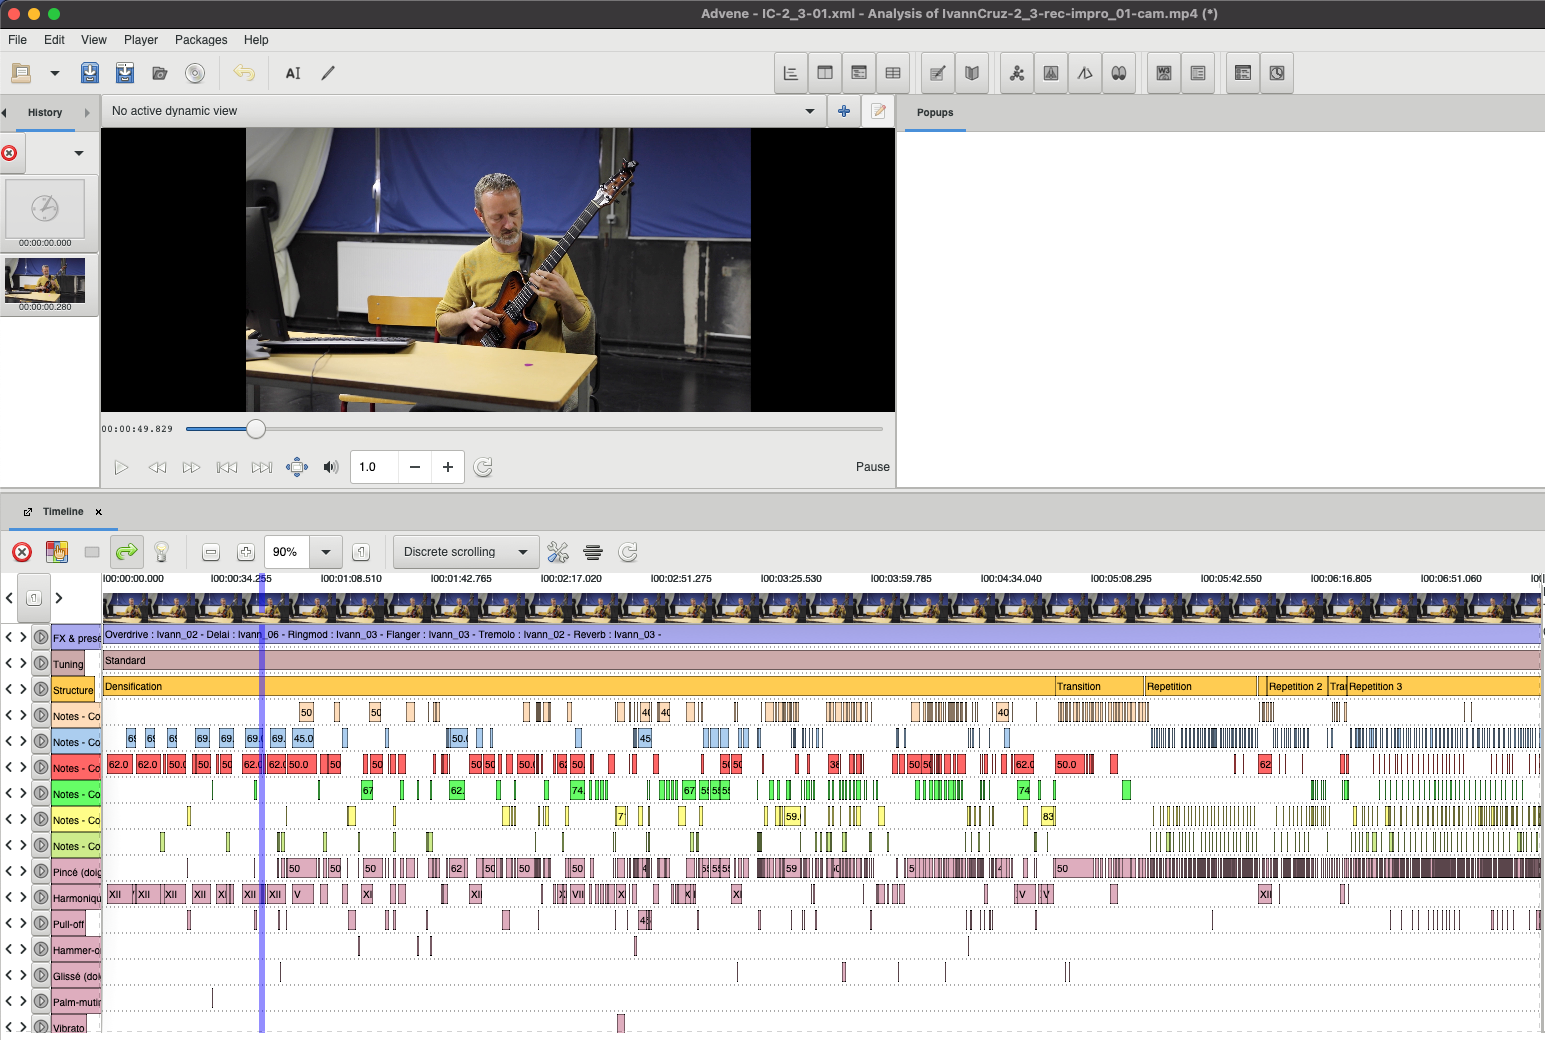
\includegraphics[width=\columnwidth]{figures/IvannCruz_2_3_1_Advene.png}
    \caption{GIHME annotations integration example in Advene software.}
    \label{fig:Ivann-2_4-timeline}
\end{figure}
%total duration of improvisation, total duration of interviews, features (onset, offset, string, fret, tuning), etc.

The global dataset provides 10 hours of guitarists improvisations (audio -hexaphonic and monophonic format- and video recordings) using an hexaphonic multi-effects as well as 4 hours and 30 minutes of interview have been transcribed.

%\begin{itemize}
%    \item synchronisation points annotation and use of script to automatically sync all the medias for a given sub-scenario. Screen video have been resampled so that it matches the camera resolution and fps rate.
    
%    \item string/fret : played fret number has been automatically inferred from hexaphonic signals using a script performing automatic pitch recognition. The result of this script is then human verified.
    
 %   \item computer vision techniques have been used and screen videos in order to capture and annotate the use of strings with effects vs strings without effect in the first scenario and activated bypasses in the second scenario.
%\end{itemize}


\section{Interviews analysis}
\label{itw_analysis}

This analysis is a first step towards understanding and characterizing how guitarists get to grips with such a system and what and how the use of hexaphonic guitar and effects alters or not their practices. 

\subsection{Biases}
The experiment introduces several biases which have to be taken into account.

The first one is the duration of the experiment. Three days per guitarist is a limited amount of time that enables the guitarists to have a good first idea of the artistic potentials of the system but not to develop a specific practice with new modes of playing for example. Guitarist number 5 clearly stated that more time would have been the solution to find more ideas for each scenario. 

\begin{quote}
    "I think I could get something out of it, but I would need more time [...]. I would need to play it everyday in order to find stuff that I like. (Guitarist 5, extract from post-improvisation interview, scénario2\_5, pers. comm.)
\end{quote}
%Alexandre Antoine

%\begin{quote}
%    "Je pense que c'est beaucoup de boulot [...]. Je ne sais pas si au final [...] ça peut me servir pour moi ce que je fais, pour l'utilisation que j'ai de la guitare. [...] Je pense que je pourrais arriver à quelque-chose, mais il faudrait beaucoup plus de temps. [...] Faudrait que j'en fasse tous les jours pour trouver un truc qui me plait.(Alexandre Antoine, extrait interview post-improvisation, scénario2\_5)"
%\end{quote}

The number of guitarists is also quite limited due to economic reasons. The analysis coming out from this dataset therefore cannot be easily generalized.  

Practice of each guitarist was partially known by the researcher and several parts of the interviews are questions related to understanding whether or not the different techniques they used were part of their practices or were induced by the system.


%
%    \begin{quote}
%        "Là comme t’alternes tu sais pas trop sur quel pied danser, donc euh […], ouais faut vraiment réinventer une façon de jouer. (extrait interview post-improvisation, scénario1\_3, Sébastien Beaumont)"
%    \end{quote}
    
%Necessity of having a practice developed enough to extract the most of hexaphony and hexaphonic processing.
%Strong tool to enhance performance of guitarists with timbral approach to guitar 

%Several of them used various techniques to simplify the complexity of the different scenarios : not a lot of techniques (tapping + tremolo) for SB, detuning of strings to obtain 2 or 3 harmonic distinct poles (RG), focused on 2 or 3 strings (PL)

\subsection{Constraints and limitations}
One of the common point to all guitarists during these experiments is that, at some point, they felt constrained. The limitations they endured were most of the time due to the configuration of the multi-effects, the configuration of the scenarios or the hexaphonic pickup behavior.

It has to be noticed that the scenarios and sub-scenarios configurations are constraints already, as they put all the guitarists in unusual situations, but most of the time the guitarists have managed to work with them and felt stimulated by them. The constraints listed above and related to scenarios' configurations are the ones where guitarists had a hard-time integrating those configuration in their improvisations.

Regarding the hexaphonic multi-effects several constraints were mentioned : the balance between the volume of dry strings and strings on which effects were applied in scenario\_1 was, for example, mentioned by guitarists 1 and 3 as being problematic (the issue was resolved by adding a dry strings volume to enhance their presence compared to the strings with effects). Some effects configurations were felt uneasy : guitarist 1 had trouble playing with different delay times when those were not rhythmically related and guitarist 5 felt that applying distorsion only on specific strings was not a natural fit for him. 

On the scenario level, all the manipulations needed to access the different individual bypasses in scenarios 2\_3, 2\_4 and 2\_5 was mentioned by guitarists 1, 4 and 5 as being not intuitive and adding a strong inertia to the whole process.
Guitarist 2 felt a strong constraint with effects distribution in scenario1\_3 and 1\_4 :
%    \begin{quote}
%        "je me retrouve un peu démuni en fait devant une configuration comme celle-là. Donc euh, j’ai mes réflexes de, de, de guitariste […] qui essaient d’aller chercher quelque-chose mais qui n’est plus là. Donc euh, oui ça essaie, ça pointe son nez, mais ça marche pas [silence]." (extrait interview post-improvisation, scénario1\_3-02, Sébastien Beaumont)
%    \end{quote}
    \begin{quote}
        "I was a bit helpless in fact with a setup like this one. [...] I have my guitarist's reflexes that try to find something but which is not there anymore. So, yeah it tries [...], but it doesn't work. (Guitarist 2, extract of post improvisation interview, scenario1\_3-02, pers. comm.)."
    \end{quote}
    %%%% Sébastien Beaumont

One last type of constraint is due to acoustic and electric behavior of the hexaphonic. Indeed cross-talk\footnote{A small amount of the sound of a vibrating string is picked up by adjacent pickups.} and transfer of a played string's vibrations to other pickups through the bridge create resonances on non-played strings. These two phenomena are particularly significant in scenario 1, where notes played on strings without effects would trigger low volume modified sounds despite no string with effects have been played.
However, these constraints were used by guitarist 2, 3 and 4 as a mode of playing in itself. 

%Alongside with this specific adaptation, it has to be noticed, that most constraints felt by guitarists regarding the scenarios' specificity were integrated and resolved along the run through the sub-scenarios. These resolutions appeared most of the times after guitarist's acceptance of the system specificities. As guitarist one stated : 
%    \begin{quote}
%        "I was a bit helpless in fact with a setup like this one. [...] I have my guitarist's reflexes that try to find something but which is not there anymore. So, yeah it tries [...], but it doesn't work. (Sébastien Beaumont, extract of post improvisation interview, scenario1\_3-02, pers. comm.)."
%    \end{quote}

%Foot controller


\subsection{Appropriation of the system}

Apart from the previous constraints (resonances on strings that haven't been played) that several guitarists turned into a mode of playing, no new modes of playing where mentioned during the interviews. As stated in the previous paragraph, this may be due partly to the short duration of these experiments.  
Likewise, apart from the constraints listed above, a good part of the system's complexity was integrated by all the guitarists.

\subsubsection{Strategies to reduce complexity}
In order to achieve this integration in such a limited amount of time, most of the guitarists used techniques to limit the complexity of the system to something they could more easily apprehend. Guitarist 3 played several improvisations using only a limited amount of prepared strings\footnote{Instrument's preparations is the process by which object are added or fixed on the string in order to modify its original timbre.} (scenario 1\_2) or a limited way to attack the strings (scenarios 2\_1, 2\_2, 2\_3). Guitarist number 2 recorded one improvisation with two different playing techniques from the beginning to end in relationship with the effects distribution of the scenario (scenario 1\_2). This choice emphasized the polyphonic effect of the scenario and help the guitarist focus on the timbre. In scenario 1\_2, guitarist 4 used preparation (a small bar of metal inserted in between the strings close to the bridge) on the three dry strings in order to bring their timbre closer to the ones of the strings with effects. The same guitarist used scordatura\footnote{The scordatura is the operation by which strings are detuned in order to go away from the original harmony of the instrument and to access different quality of timbre as it evolves with string tension.} right from the beginning (scenario 1\_1) to limit the harmonic possibilities:
    \begin{quote}
        "It appeared to me as a way, in this chaos of the low strings [strings with effects, ed's note], to try to find an organization clearer for me. (Guitarist 4, extract of post improvisation interview, scenario1\_1, pers. comm.)."
    \end{quote}
In this improvisation, the standard tuning of the guitar, E-A-D-G-B-e, became E-A-D-A-A-e (the D string was left unused during all the improvisation). 

\subsubsection{Respect of the guitarist practice}
From the guitarists points of view, this system wasn't a new instrument as their practices didn't have to be drastically modified but "only" adapted :
    \begin{quote}
        "It doesn't question the pratice. The practice, it stays, it exists. However, it reconsiders it, in the sens where, as new things happen, you have to adapt. (Guitarist 2, extract of post improvisation interview, scenario2\_5, pers. comm.)."
    \end{quote}
The same guitarist develops this idea further :
    \begin{quote}
        "It's a system who forces you to look deeply at the instrument for ways to adapt, even if it is a material that I know. I mean, all this effects, I've already used them in my life. They are part of the guitarist's landscape. And despite all that, the fact to use them in hexaphony, you rethink the effects differently too. You rethink, you adapt your playing, an interaction takes place (Guitarist 2, extract of post improvisation interview, scenario2\_5, pers. comm.)."
    \end{quote}    

Those two quotes emphasize the analog-style of this system in which the guitarist's gesture was kept from being reduced. Systems such as guitar synthesizer (as well as a large part of digital luthery instruments) performs digital reduction of guitarist's gesture by transforming it into pitch and intensity. All the subtlety acquired by the guitarist during its years of practice is then limited to the notes he plays and their intensities.
The fact that the system presented here kept the subtlety of the guitarists' practice helped them into the appropriation process.

Following this idea, it clearly appears that, during these three days, practices that already make use of techniques to develop polyphonic or multitimbral approaches of the guitar were enhanced by this system. 
Guitarist 3 who extensively used preparations during its improvisation pointed out at several moments the gain of clarity due to the hexaphony. Indeed as not all preparations fits a specific monophonic effect, extra manipulations would be needed in order to apply it to specific preparations. With the possibility to configure independently each string, guitarists who use preparations can prepare them and their associated effects in advance, without the obligation to think up their removal or installation.

Guitarist 4 tends to approach its instrument specifically in timbre terms by the use of different types of attacks or by the use of scordatura. The latter, to him, finds a perfect continuity in the use of string-independent effects as it can emphasize the different timbres obtained by the reduction of the string tension. 


%Ça remet pas en cause la pratique. Ta pratique, elle reste, elle existe. Par contre, ça la remet en question dans le sens où, comme il se passe d’autres choses, il faut que tu t’adaptes

%c’est un dispositif qui euh, qui te force quand même à chercher sur l’instrument des moyens d’adaptation, alors que c’est un matériau finalement que je connais. Enfin, tous ces effets-là, je les avais déjà utilisés dans ma vie. Ils font partis du paysage euh, du guitariste. Et malgré tout, le fait de les utiliser en, en hexaphonie comme ça ben, [court silence] tu repenses aussi les effets différemment, tu repenses, t’adaptes ton jeu, enfin y’a une interaction qui se passe.

\section{Conclusion}
This paper presents a novel dataset including improvisations of 5 different guitarists using a system made out of an hexaphonic guitar and an hexaphonic multi-effects audio program. Such a system enables them to apply string-independent effects. This dataset was built to try to understand how the hexaphonic, or string-independent, audio processing affects the guitarists' practices of their instrument and how the possibilities of hexaphonic audio effects could be integrated into their practices. The dataset is made out of 10 hours of audio and video recordings of improvisation, 4 hours and 30 minutes of transcribed interviews and annotations such as the played notes, the used tuning(s) and effects activation segments.
The analysis of the interviews shows that despite the obvious complexity and constraints of the system, appropriation phenomena appears through several ways : the guitarists develop strategies to reduce the complexity; their practices, as they remained unchanged, help them to embrace the new potentials; as hexaphonic audio processing emphasizes polyphony and multitimbrality, therefore practices that were already integrating such techniques found a natural fit to the system. 

The interviews discourses study gives several ideas of what's at stake when a guitarist uses a string-independent audio effects processing system. These ideas need to be developed and documented in order to give strong understanding of the guitarists' practices' mutations. The annotations and the visualization, which haven't been much used yet, will be enriched (chord, interval annotations, string/fret visualisation, etc.) and integrated in the analysis process.







%%%%%%%%%%%%%%%%%%%% FROM TEMPLATE
%\section{Page size and format}
%\label{sec:page_size}
%The SMC 2022 proceedings will be formatted as portrait \underline{A4-size papers (21.0~cm x 29.7~cm)}. All material on each page should fit within a rectangle of 17.2~cm x 25.2~cm, centered on the page, beginning 2.0~cm from the top of the page and ending with 2.5~cm from the bottom. The left and right margins should be 1.9~cm. The text should be in two 8.2~cm columns with a 0.8~cm gutter. All text must be in a two-column format, and justified.
%
%Papers should be between 4 and 8 pages, written in English, and not previously published. Papers must be submitted as PDF documents generated using the provided \LaTeX{} or Word templates.
%
%
%\section{Typeset Text}\label{sec:typeset_text}
%
%\subsection{Normal or Body Text}
%\label{subsec:body}
%Please use a 10~pt (point) Times font. Use sans-serif or non-proportional fonts only for special purposes, such as distinguishing source code.
%
%The first paragraph in each section should not be indented, 
%but all other paragraphs should be.
%
%\subsection{Title and Authors}
%The title is 16~pt Times, bold, caps, upper case, centered. Authors' names are centered. The lead author's name is to be listed first (left-most), and the co-authors' names after. If the addresses for all authors are the same, include the address only once, centered. If the authors have different addresses, put the addresses, evenly spaced, under each authors' name.
%
%\subsection{First Page Copyright Notice}
%Please leave the copyright notice exactly as it appears in the lower left-hand corner of the first page. Make sure to update the first author’s name in the copyright notice, accordingly. It is set in 8~pt Times.
%
%\subsection{Page Numbering, Headers and Footers}
%Do not include headers, footers or page numbers in your submission. These will be added electronically at a later stage, when the publications are assembled.
%
%\section{Headings}
%First level headings are in Times 12~pt bold, centered with 1 line of space above the section head, and 1/2 space below it.
%For a section header immediately followed by a subsection header, the space should be merged.
%
%\subsection{Second Level Headings}
%Second level headings are in Times 10~pt bold, flush left, with 1 line of space above the section head, and 1/2 space below it. The first letter of each significant word is capitalized.
%
%\subsubsection{Third Level Headings}
%Third level headings are in Times 10~pt italic, flush left, with 1/2 line of space above the section head, and 1/2 space below it. The first letter of significant words is capitalized.
%
%Using more than three levels of headings is strongly discouraged.
%
%
%
%
%
%\section{Floats and equations}
%
%\subsection{Equations}
%Equations should be placed on separated lines and numbered. The number should be on the right side, in parentheses.
%\begin{equation}
%r=\sqrt[13]{3}
%\label{eq:BP}
%\end{equation}
%Always refer to equations like this: ``Equation (\ref{eq:BP}) is of particular interest because...''
%
%\subsection{Figures, Tables and Captions}
%\begin{table}[t]
% \begin{center}
% \begin{tabular}{|l|l|}
%  \hline
%  String value & Numeric value \\
%  \hline
%  Moin! SMC & 2022 \\
%  \hline
% \end{tabular}
%\end{center}
% \caption{Table captions should be placed below the table,  like this.}
% \label{tab:example}
%\end{table}
%
%All artwork must be centered, neat, clean and legible. Figures should be centered, neat, clean
%and completely legible. All lines should be thick and dark enough for purposes of reproduction. Artwork should not be hand-drawn. The proceedings will be distributed in electronic form only, therefore color figures are allowed. However, you may want to check that your figures are understandable even if they are printed in black-and-white.
%
%
%Numbers and captions of figures and tables always appear below the figure/table.
%Leave 1 line space between the figure or table and the caption.
%Figure and tables are numbered consecutively. 
%Captions should be Times 10pt. Place tables/figures in the text as close to the reference as possible, 
%and preferably at the top of the page.
%
%Always refer to tables and figures in the main text, for example: ``see Fig. \ref{fig:example} and \tabref{tab:example}''.
%Figures and tables may extend across both columns to a maximum width of 17.2cm.
%
%Vectorial figures are preferred, e.g., eps. When using \texttt{Matlab}, export using either (encapsulated) Postscript or PDF format. In order to optimize readability, the font size of text within a figure should be no smaller than
%that of footnotes (8~pt font-size). If you use bitmap figures, make sure that the resolution is high enough for print quality. 
%
%\begin{figure}[t]
%\centering
%
\includegraphics[width=0.6\columnwidth]{figure}
%\caption{Figure captions should be placed below the figure, 
%exactly like this.\label{fig:example}}
%\end{figure}
%
%
%\subsection{Footnotes}
%You can indicate footnotes with a number in the text \footnote{This is a footnote example.},
%but try to work the content into the main text.Use 8~pt font-size for footnotes.  Place the footnotes at the bottom of the page 
%on which they appear. Precede the footnote with a 0.5~pt horizontal rule.
%
%\section{Citations}
%All bibliographical references should be listed at the end, inside a section named ``REFERENCES''. References must be numbered in order of appearance. You should avoid listing references that do not appear in the text.
%
%Reference numbers in the text should appear within square brackets, such as in~\cite{Someone:00} or~\cite{Someone:00,Someone:04,Someone:09}. The reference format is the standard IEEE one. We highly recommend you use BibTeX 
%to generate the reference list.
%
%\section{Conclusions}
%Please, submit full-length papers. Submission is fully electronic and automated through the Conference Web Submission System. \underline{Do not} send papers directly by e-mail.


\begin{acknowledgments}
At the end of the Conclusions, acknowledgements to people, projects, funding agencies, etc. can be included after the second-level heading  ``Acknowledgments'' (with no numbering).
\end{acknowledgments} 

%%%%%%%%%%%%%%%%%%%%%%%%%%%%%%%%%%%%%%%%%%%%%%%%%%%%%%%%%%%%%%%%%%%%%%%%%%%%%
%bibliography here
\bibliography{GIHME-SMC2022-bibliography}

\end{document}
